\documentclass[9pt]{beamer}
\usepackage{etex}
\usepackage{pres}
\usepackage{gensymb}

\makeatletter
\newif\if@restonecol
\makeatother
\let\algorithm\relax
\let\endalgorithm\relax
\usepackage[ruled,vlined,linesnumbered,lined]{algorithm2e}

\usefonttheme[onlymath]{serif}

\newcommand{\sseq}[1]{{\color{blue}\seq{#1}}}

\newcommand{\poly}{\textrm{poly}}
\newcommand{\Rat}{\mathbb{Q}}

\providecommand{\DontPrintSemicolon}{\dontprintsemicolon}

\pgfdeclareimage[width=6cm]{cps}{cps}

\hypersetup{
  pdftitle={Formal Verification: Projects},
  pdfauthor={Umang Mathur}}

\title{An Optimization Approach for Solving Reachability in Cyber-Physical Systems}
\author{Umang Mathur \and Atul Sandur}
  

\institute[CS, UIUC] {\vspace{0.1cm} 
  Department of Computer Science\\
  University of Illinois, Urbana Champaign} 

  
\date{\today}

%%%%%%%%%%%%%%%%%%%%%%%%%%%%%%%%%%%%%%%%%%%%%%%%%%%%%%%%%%%%%%%%%%%%%%%%%%%%%%%%%%%%%%%%%% 
%%    Main Body
%%%%%%%%%%%%%%%%%%%%%%%%%%%%%%%%%%%%%%%%%%%%%%%%%%%%%%%%%%%%%%%%%%%%%%%%%%%%%%%%%%%%%%%%%%

\begin{document}

\frame{\titlepage}

\frame{\frametitle{Outline}
\tableofcontents}

\section{Introduction}
 \frame{
  \frametitle{Cyber-Physical Systems (CPS)}
  \begin{itemize}
    \item Cyber-Physical systems are engineered systems that depend upon the integration of
        \begin{itemize}
            \item computational algorithms, and 
            \item physical components 
        \end{itemize}
    \vspace{0.25in}
    \item Diverse applications:
        \begin{itemize}
            \item Healthcare
            \item Aerospace, Aeronautics
            \item Chemical processes
            \item Transportation
            \item Energy sector
        \end{itemize}
  \end{itemize}
}
   

\frame{
  \frametitle{Cyber-Physical Systems (CPS)}
  \begin{center}
    \pgfuseimage{cps} 
  \end{center}
}

\frame{
  \frametitle{Hybrid Automata: Modelling, Analysis and Synthesis of CPS}
  \begin{itemize}
  \item
    Introduced by Alur et al. to model hybrid systems
  \item
    Quite expressive, but \blue{undecidable} verification (reachability)
    problems  
  \item
    Decidable subclasses exists, e.g.
    \begin{itemize}
    \item 
      \blue{Timed Automata} ({\footnotesize Alur, and Dill}),
    \item 
      \blue{Initialized Rectangular Hybrid automata} ({\footnotesize Henzinger
        et al.}), 
 %   \item 
 %     \blue{Multi-Mode Systems} ({\footnotesize Alur, Trivedi, Wojtczak})   
    \end{itemize}
    \item Most verification techniques rely on exhaustive exploration of state space using finite bisimulations
%  \item 
 %   \blue{Tool support}: \textsc{HyTech}, \textsc{PHAV}er, \textsc{Uppaal}
  \end{itemize}
  \pause
    \begin{figure}
  \begin{center}
    \scalebox{0.8}{
    \begin{tikzpicture}[->,>=stealth',shorten >=1pt,auto,semithick]
      \tikzstyle{every state}=[fill=blue!30,minimum size=3em,rounded rectangle]
      
      \node[state] at (0, 0) (m0) {$\begin{array}{c}
          \mbox{\bf Off} \\ \dot{T} = -0.1T \\ T \geq 18 \end{array}$};
      
      \node[state] at (7, 0) (m1) {$\begin{array}{c} \mbox{\bf On} \\ \dot{T} = 5-0.1T \\ T \leq 22 \end{array}$};
     % \pause
  
      \path (m0) edge[bend left] node {$T < 19$} (m1);
      
      
      \path (m1) edge[bend left] node {$T > 21$} (m0);
      %\path (m0) edge node[] {$x_2 > 0, b$} (m2);
      
      %\path (m2) edge node[] {$ x_1 < 22, c$} (m3);
      %\path (m1) edge node[] {$d$} (m3);
   
      %\path (m3) edge [loop above] node[] {$e$} (m3);
    \end{tikzpicture}
  }
\end{center}
\label{fig:sha}
  \caption{Modelling a smart heater as a Hybrid Automata} 
\end{figure}
 
}

\section{Verification and Testing of Hybrid Automata}
\frame{\tableofcontentscurrent}

\frame{
  \frametitle{Reachability in Hybrid Systems}
  Safety Critical Systems :
    \begin{itemize}
        \item Nuclear reactors
        \item Chemical plants
        \item Aeronautics/Automobiles
    \end{itemize}
    It is therefore important to have certain safety guarantees for such systems

    \vspace{0.2in}
    Checking reachability of certain states, thus, is a natural question to ask
    \begin{itemize}
        \item Can reach some error state ?
        \item How to reach ?
            \begin{itemize}
                \item input ?
                \item path ? (non-determinism)
            \end{itemize}
    \end{itemize}

    \vspace{0.2in}
    Other interesting applications:
    \begin{itemize}
        \item Motion planning
    \end{itemize}
        
%%  \begin{center}
%%    \scalebox{0.8}{  \begin{tikzpicture}[node distance=1cm]
      \node[loc,label=below:$m_1$] (p4) at (0,-2.5) {$\begin{matrix} \dot{T_1} =
          -2 \\ \dot{T_2} = 3 \end{matrix}$};
      \node[loc,label=below:$m_2$] (p5) at (3,-2.5){$\begin{matrix} \dot{T_1} = -1 \\ \dot{T_2} = -1 \end{matrix}$};
    \node[loc,label=below:$m_3$] (p6) at (6,-2.5){$\begin{matrix} \dot{T_1} = -1 \\ \dot{T_2} = 3 \end{matrix}$};
    \node[loc,label=below:$m_4$] (p7) at (0,-5) {$\begin{matrix} \dot{T_1} = 2 \\ \dot{T_2} = -2 \end{matrix}$};
    \node[loc,label=below:$m_5$] (p8) at (3,-5){$\begin{matrix} \dot{T_1} = 2 \\ \dot{T_2} = -1 \end{matrix}$};
    \node[loc,label=below:$m_6$] (p9) at (6,-5){$\begin{matrix} \dot{T_1} = 2 \\ \dot{T_2} = 3 \end{matrix}$};
  \end{tikzpicture}
}
%%  \end{center}
%%  
%%  \vfill
%%
%%  \blue{Safe Schedulability Problem:} Does there exist a \blue{switching schedule} using these \blue{modes}
%%    such that the temperatures stay in \blue{comfortable region}? 
}

\subsection{Example}

\frame{
    \frametitle{Robotic Motion Planning}
    
    \vspace{-0.2in}
    \begin{figure}%{l}{0pt}%[0.4\textwidth]
%\begin{center}
  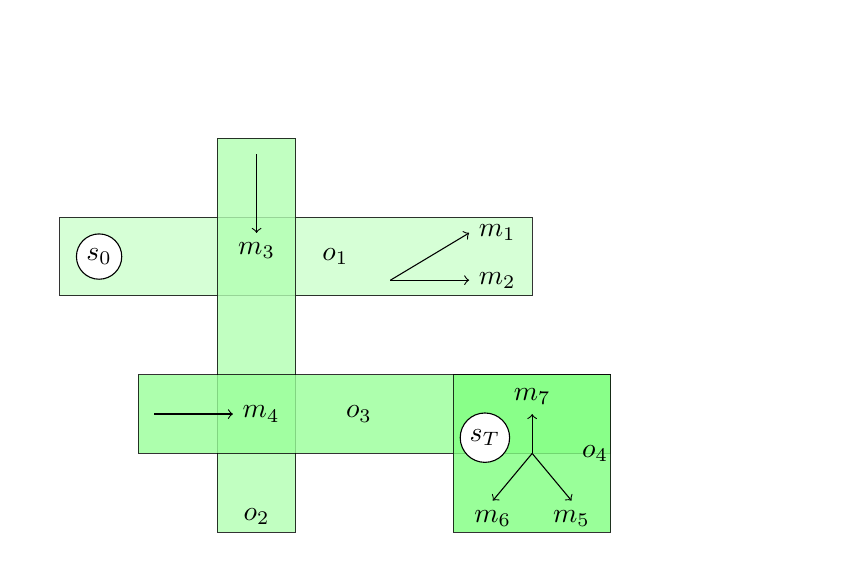
\begin{tikzpicture}
  \tikzstyle{every state}=[fill=gray!20!white,shape=rounded rectangle]
  
    \draw [fill=green!20, opacity=0.8] (0,0) rectangle (6,1);
    \node at (3.5, 0.5) {$o_1$};
    \node[fill=white!80, circle,inner sep=0.2em, draw] at (0.5, 0.5) {${\color{black}s_0}$};
    \draw[->] (4.2, 0.2) -- (5.2, 0.8) node[right] {$m_1$};
    \draw[->] (4.2, 0.2) -- (5.2, 0.2) node[right] {$m_2$};
    
    \draw [fill=green!30, opacity=0.8] (2,2) rectangle (3,-3);
    \node at (2.5, -2.8) {$o_2$};
    \draw[->] (2.5, 1.8) -- (2.5, 0.8) node[below] {$m_3$};
    
    \draw [fill=green!40, opacity=0.8] (1, -1) rectangle (7, -2);
    \node at (3.8, -1.5) {$o_3$};
    \draw[->] (1.2, -1.5) -- (2.2, -1.5) node[right] {$m_4$};
    
    \draw [fill=green!50, opacity=0.8] (5, -1) rectangle (7, -3);
    \node at (6.8, -2) {$o_4$};
    \draw[->] (6, -2) -- (6.5, -2.6) node[below] {$m_5$};
    \draw[->] (6, -2) -- (5.5, -2.6) node[below] {$m_6$};
    \draw[->] (6, -2) -- (6, -1.5) node[above] {$m_7$};
    \node[fill=white,circle,inner sep=0.2em, draw] at (5.4, -1.8)
    {${\color{black}s_T}$};
    
	\draw [dashed, draw=white] (6.6, 1.4) rectangle (7.4, -0.4);
    \draw [dashed, draw=white] (2.1, 3.4) rectangle (2.9, 2.6);
    \draw [dashed, draw=white] (-0.4, -1.1) rectangle (0.4, -1.9);
	\draw [dashed, draw=white] (7.6, -2.9) rectangle (9.9, -1.1);
      
  \end{tikzpicture}                        
%\end{center}
  \caption{Robotic motion planning problem modelled as a reachability question}
  \label{fig:robocop}
\end{figure}


    \begin{itemize}
        \item Can a bot enter $o4$ starting from some point in region $o1$ 
    \end{itemize}
}


\section{Singular Hybrid Automata: Syntax and Semantics}

\frame{
	\frametitle{Syntax of SHA}
    \begin{block}{Syntax : Singular Hybrid Automata (SHA)}
	A singular hybrid automaton is a tuple 
    \blue{$\Hh = (M, M_0, \Sigma, X, \Delta, I, F)$}
    %\blue{$\Hh = (M, M_0, X, \Delta, I, F)$}
	where
	\begin{itemize}
		\item $M$ is a finite set of control {\color{blue}{modes}} and $M_0 \subseteq M$, 
		\item $\Sigma$ is a finite set of {\color{blue}actions},
		\item $X$ is an (ordered) set of {\color{blue}variables}, 
		%\item $\Delta \subseteq M \times \poly(X) \times 2^{X} \times M$ is the {\color{blue}transition relation}, 
		\item $\Delta \subseteq M \times \poly(X) \times \Sigma \times 2^{X} \times M$ is the {\color{blue}transition relation}, 
		\item $I: M \to \poly(X)$  is the {\color{blue}mode-invariant} function, and
		\item $F: M \to \Rat^{|X|}$ is the mode-dependent {\color{blue}flow function} characterizing the rate of each variable in each mode.
	\end{itemize}
    \end{block}

    \begin{figure}
    \begin{center}
        \scalebox{0.8}{
            \begin{tikzpicture}[->,>=stealth',shorten >=1pt,auto,semithick]
                \node[loc, label=below:$m_0$, label=left:
                $\begin{matrix}
                    x_1 - 3x_2 \leq 10 \\
                    x_2 > -3
                \end{matrix}$] (m0) at (0,-2.5) {
                    $\begin{matrix}
                        \dot{x_1} = -2 \\ 
                        \dot{x_2} = 3 
                    \end{matrix}$
                };
                \node[loc,label=below:$m_1$, label=right:$2x_1 + 3x_2 \leq 5$] (m1) at (5,-2.5) {
                    $\begin{matrix}
                        \dot{x_1} = 0 \\ 
                        \dot{x_2} = -2
                    \end{matrix}$
                };
            
                \path (m0) edge[bend left] node {$a, \, x_1 + 2x_2 \leq 19$} node[below] {$\{x_2\}$} (m1);
                \path (m1) edge[bend left]  node[above] {$b, \, x_1 > -21$} node[below] {$\{x_1, x_2\}$}(m0);
            \end{tikzpicture}
        }
    \end{center}
    \label{fig:sha-syntax}
    \caption{Example SHA} 
\end{figure}

	
}

\frame{
	\frametitle{Semantics of SHA}
	\begin{itemize}
	\item \blue{Configuration} $(m, \nu)$, $m \in M$, $\nu \in \mathbb{R}^{\lvert X \rvert}$
    \item \blue{Timed action} $(t, a)$, $t \in \mathbb{R}^{\geq 0}$ and $a \in \Sigma$ 
	\item \blue{Transition} $((m, \nu) (t, a) (m', \nu'))$
%%%%	\begin{itemize}
%%%%        \item $(m, g, a, \mathcal{R}, m') \in \Delta$
%%%%            \begin{itemize}
%%%%                \item guard $g \in$ poly$(X)$
%%%%                \item $a \in \Sigma$
%%%%                \item reset set $\mathcal{R} \in 2^X$ 
%%%%            \end{itemize}
%%%%		\item For all $\hat{\nu} \in [\nu, \nu + t\cdot F(m)]$, $\hat{\nu} \in I(m)$ (Invariant)
%%%%        \item $\hat{\nu}' \in g$, where $\hat{\nu}' = \nu + t\cdot F(m)$
%%%%        \item   $\nu'(x_i)=
%%%%                    \begin{cases}
%%%%                        \nu(x_i) & x_i \not\in \mathcal{R}\\
%%%%                        0 & \text{ otherwise }
%%%%                    \end{cases}
%%%%                $
%%%%		\item $\nu' \in I(m')$ (Invariant)
%%%%	\end{itemize} 
	\item A \blue{run} is a sequence of transitions $(m_0, \nu_0) (t_1, a_1)
	(m_1, \nu_1) (t_2, a_2) \cdots$
	\end{itemize}

    \begin{figure}
    \begin{center}
        \scalebox{0.8}{
            \begin{tikzpicture}[->,>=stealth',shorten >=1pt,auto,semithick]
                \node[loc, label=below:$m_0$, label=left:
                $\begin{matrix}
                    x_1 - 3x_2 \leq 10 \\
                    x_2 > -3
                \end{matrix}$] (m0) at (2.5,2.5) {
                    $\begin{matrix}
                        \dot{x_1} = -2 \\ 
                        \dot{x_2} = 3 
                    \end{matrix}$
                };
                \node[loc,label=below:$m_1$, label=right:$2x_1 + 3x_2 \leq 5$] (m1) at (7.5,2.5) {
                    $\begin{matrix}
                        \dot{x_1} = 0 \\ 
                        \dot{x_2} = -2
                    \end{matrix}$
                };
            
                \path (m0) edge[bend left] node {$a, \, x_1 + 2x_2 \leq 19$} node[below] {$\{x_2\}$} (m1);
                \path (m1) edge[bend left]  node[above] {$b, \, x_1 > -21$} node[below] {$\{x_1, x_2\}$}(m0);

            \pause 

            \only<8, 9, 12>{
                \node[yloc, label=below:$m_0$, label=left:
                $\begin{matrix}
                    x_1 - 3x_2 \leq 10 \\
                    x_2 > -3
                \end{matrix}$] (m0) at (2.5,2.5) {
                    $\begin{matrix}
                        \dot{x_1} = -2 \\ 
                        \dot{x_2} = 3 
                    \end{matrix}$
                };
            }

            \only<10, 11>{
                \node[yloc,label=below:$m_1$, label=right:$2x_1 + 3x_2 \leq 5$] (m1) at (7.5,2.5) {
                    $\begin{matrix}
                        \dot{x_1} = 0 \\ 
                        \dot{x_2} = -2
                    \end{matrix}$
                };
            }

    \node[stloc, label=left:
        $\begin{matrix} 
            x_1\\
            x_2
        \end{matrix}$,
        label=below:$m_0$] (s0) at (0,0) {$\begin{matrix} 0 \\ 0 \end{matrix}$};

    \pause
    \node[stloc, label=below:$m_0$] (s1) at (2,0) {$\begin{matrix} -2 \\ 3
      \end{matrix}$};  
    \draw[trans](s0) --node[midway,above]{$1$}  (s1);
    
    \pause
    \node[stloc, label=below:$m_1$] (s2) at (4,0) {$\begin{matrix} -2 \\ 0
      \end{matrix}$};  
    \draw[trans](s1) --node[midway,above]{$a$}  (s2);
    
    \pause
    \node[stloc, label=below:$m_1$] (s3) at (6,0) {$\begin{matrix} -2 \\ -1
      \end{matrix}$};  
    \draw[trans](s2) --node[midway,above]{$0.5$}  (s3);
    \pause
    \node[stloc, label=below:$m_0$] (s4) at (8,0) {$\begin{matrix} 0 \\ 0
      \end{matrix}$};  
    \draw[trans](s3) --node[midway,above]{$b$}  (s4);
    \draw[trans](s4) --node[midway,above]{$ \cdots$}  (10,0) ;


            \end{tikzpicture}
        }
    \end{center}
    \label{fig:sha-semantics}
    \caption{Example run in a SHA} 
\end{figure}

	
}

\frame{
    \frametitle{Modelling Robot Motion Planning Using SHA}    

    \vspace{-0.2in}
    \begin{figure}%{l}{0pt}%[0.4\textwidth]
\begin{center}
  \begin{tikzpicture}
  \tikzstyle{every state}=[fill=gray!20!white,shape=rounded rectangle]
  
    \draw [fill=green!20, opacity=0.8] (0,0) rectangle (6,1);
    \node at (3.5, 0.5) {$o_1$};
    \node[fill=white!80, circle,inner sep=0.2em, draw] at (0.5, 0.5) {${\color{black}s_0}$};
    \draw[->] (4.2, 0.2) -- (5.2, 0.8) node[right] {$m_1$};
    \draw[->] (4.2, 0.2) -- (5.2, 0.2) node[right] {$m_2$};
    
    \draw [fill=green!30, opacity=0.8] (2,2) rectangle (3,-3);
    \node at (2.5, -2.8) {$o_2$};
    \draw[->] (2.5, 1.8) -- (2.5, 0.8) node[below] {$m_3$};
    
    \draw [fill=green!40, opacity=0.8] (1, -1) rectangle (7, -2);
    \node at (3.8, -1.5) {$o_3$};
    \draw[->] (1.2, -1.5) -- (2.2, -1.5) node[right] {$m_4$};
    
    \draw [fill=green!50, opacity=0.8] (5, -1) rectangle (7, -3);
    \node at (6.8, -2) {$o_4$};
    \draw[->] (6, -2) -- (6.5, -2.6) node[below] {$m_5$};
    \draw[->] (6, -2) -- (5.5, -2.6) node[below] {$m_6$};
    \draw[->] (6, -2) -- (6, -1.5) node[above] {$m_7$};
    \node[fill=white,circle,inner sep=0.2em, draw] at (5.4, -1.8)
    {${\color{black}s_T}$};

    \pause
    
	\node[state,fill=gray!20, scale=0.7] at (7, 1) (m1) {$m_1$};
	\node[state,fill=gray!20, scale=0.7] at (7, 0) (m2) {$m_2$};
	\draw [dashed] (6.6, 1.4) rectangle (7.4, -0.4);
	\path[->] (m1) edge[bend left] (m2);
     \path[->] (m2) edge[bend left] (m1);
	
	\node[state, fill=gray!20, scale=0.7] at (2.5,3) (m3) {$m_3$} ;
    \draw [dashed] (2.1, 3.4) rectangle (2.9, 2.6);
    
    \node[state, fill=gray!20, scale=0.7] at (0,-1.5) (m4) {$m_4$} ;
    \draw [dashed] (-0.4, -1.1) rectangle (0.4, -1.9);
    
	\node[state, fill=gray!20, scale=0.7] at (8,-1.5) (m5) {$m_5$} ;
	\node[state, fill=gray!20, scale=0.7] at (9.5,-1.5) (m6) {$m_6$} ;
	\node[state, fill=gray!20, scale=0.7] at (8.75,-2.5) (m7) {$m_7$} ;
	\draw [dashed] (7.6, -2.9) rectangle (9.9, -1.1);
	\path[->] (m5) edge (m6);
    \path[->] (m6) edge (m7);
    \path[->] (m7) edge  (m5);
      
    
    

  \end{tikzpicture}                        
\end{center}
  \caption{Robotic motion planning problem: Modelling as a SHA}
  \label{fig:robocop}
\end{figure}

}

\frame{
    \frametitle{Modelling Robot Motion Planning Using SHA}    

    \vspace{-0.2in}
    \begin{figure}[t]

  \begin{center}
     \scalebox{0.9}{
    \begin{tikzpicture}
      \tikzstyle{every state}=[fill=gray!20!white,minimum size=2em,shape=rounded rectangle]
      

      \node[state,fill=gray!20] (m1) {$m_1$};
      \node[state,fill=gray!20] at (0, -2) (m2) {$m_2$};
      \draw [dashed] (-0.5, 0.5) rectangle (0.5, -2.5) node[right] {$o_1$};
      \node at (0, -2.8) {$0{<} x {<} 6$};
      \node at (0, -3.1) {$0 {<} y {<} 1$};
      
      
      \node[state, fill=gray!20] at (2.5,0) (m3) {$m_3$} ;
      \draw [dashed] (2, 0.5) rectangle (3, -0.5) node[right]{$o_2$} ;
      \node at (2.5, -0.8) {$2{<} x {<} 3$};
      \node at (2.5, -1.1) {$-3 {<} y {<} 3$};

      \node[state, fill=gray!20] at (5.5,0) (m4) {$m_4$} ;
      \draw [dashed] (5, 0.5) rectangle (6, -0.5) node[right]{$o_3$};
      \node at (5.5, -0.8) {$1{<} x {<} 7$};
      \node at(5.5, -1.1) {$-2 {<} y {<} {-}1$};

      \node[state, fill=gray!20] at (8,0) (m5) {$m_5$} ;
      \node[state, fill=gray!20] at (10,0) (m6) {$m_6$} ;
      \node[state, fill=gray!20] at (9,-2) (m7) {$m_7$} ;
      \draw [dashed] (7.5, 0.5) rectangle (10.5, -2.5) node[right]{$o_4$};
      \node at (9, -2.8) {$5 {<} x {<} 7, -3 {<} y {<} -1$};

     \path[->] (m1) edge[bend left] node [right] {$\top$}  (m2);
     \path[->] (m2) edge[bend left] node [left] {$\top$}  (m1);

     \path[->] (m1) edge node [above] {$2 {<} x {<} 3$}  (m3);
     \path[->] (m3) edge node [above] {$-2 {<} y {<} -1$}  (m4);

     \path[->] (m4) edge node [above] {$5 {<} x {<} 7$}  (m5);

    \path[->] (m5) edge node [above] {$\top$}  (m6);
    \path[->] (m6) edge node [right] {$\top$}  (m7);
    \path[->] (m7) edge node [left] {$\top$}  (m5);
    \end{tikzpicture}
    }
  \end{center}
\caption{Singular Hybrid Automaton for robotic motion planning example}
\label{fig:wsha}
\end{figure}


}

\subsection{Reachability}

\frame{
  \frametitle{Reachability in SHA}
  \begin{block}{Configuration Reachability Problem}
    Given a \blue{singular hybrid automaton $\mathcal{A}$}, a set of starting configurations $\mathcal{S}$, and a set of target configurations $\mathcal{T}$, decide whether there exists a
    \begin{itemize}
        \item \blue{finite} run 
        \item starting from some starting from some $(m, \nu) \in \mathcal{S}$, and
        \item ending in some $(m', \nu') \in \mathcal{T}$
    \end{itemize}
  \end{block}
\pause

  \vspace{0.4in}
  \begin{theorem}[Henzinger et. al., '98]
      Configuration reachability problem is undecidable for 3 or more continuous variables. 
  \end{theorem}
}

\section{Future Work}
\frame{
	\frametitle{Summary and Future Work}

	\begin{itemize}
		\item Future work
	\end{itemize}
}

\frame{
\frametitle{}
	\begin{center}

        \font\endfont = cmss9 at 15.40mm
        \endfont 
        \baselineskip 20.0mm

        Thank You !

      \end{center}    
}



%\nocite{*}

%\bibliographystyle{plain}
%\bibliography{papers}

\end{document}
